\documentclass[11pt]{article}
\usepackage[ left=2cm, top=3cm, a4paper, text={17cm, 24cm}]{geometry}
\usepackage{graphicx} % Required for inserting images
\usepackage{pdflscape}
\usepackage[T1]{fontenc}
\usepackage{times}
\usepackage[utf8]{inputenc}
\usepackage[czech]{babel}
\usepackage{hyperref}
\usepackage{amsthm}
\usepackage{amsmath}
\usepackage{array}
\usepackage{float}
\usepackage{multirow}
\usepackage{multicol}
\usepackage[czech, ruled, linesnumbered, noline, longend]{algorithm2e}
\SetNlSty{textbf}{}{:}
%% TO DO: 

\begin{document}
\catcode`\-=12
\begin{titlepage}
\begin{center}
    \Huge
	\textsc{Vysoké učení technické v~Brně}\\
    \huge
	{\textsc{Fakulta informačních technologií }}\\
	
	\vspace{\stretch{0.382}}
	\LARGE
	Typografie a publikování\,--\,3. projekt\\
	\Huge
    Tabulky a obrázky\\
	
	\vspace{\stretch{0.618}}
\end{center}
{\Large 4. apríla 2024 \hfill
Jaroslav Mervart (xmervaj00)}
\end{titlepage}

\section{Úvodní strana}
Název práce umístěte do zlatého řezu a nezapomeňte uvést dnešní datum a vaše jméno a příjmení.
\section{Tabulky}
Pro sázení tabulek můžeme použít buď prostredí \texttt{tabbing} nebo prostředí \texttt{tabular}.
\subsection{Prostředí \texttt{tabbing}}
Pri použití \texttt{tabbing} vypadá tabulka následovně:
%% TABULKA
\begin{tabbing}
\verb|\pushtabs|\qquad\quad \= Cena \quad \= Mnozstvi \kill
\textbf{Ovoce} \> \textbf{Cena} \> \textbf{Množství} \\
Jablka \> 20,- \> 3\,kg \\
Hrušky \> 25,- \> 2,5\,kg \\
Vodní melouny \> 35,- \> 1\,kus \\
\end{tabbing}

\noindent Toto prostředí se dá také použít pro sázení algoritmů, ovšem vhodnejší je použít prostředí \texttt{algorithm} nebo \texttt{algorithm2e} (viz sekce \ref{Algoritmy}).

\subsection{Prostředí \texttt{tabular}}
Další možností, jak vytvořit tabulku, je použít prostředí \texttt{tabular}. Tabulky pak budou vypadat takto\footnote{Kdyby byl problém s~\texttt{cline}, zkuste se podívat třeba sem: \href{http://www.abclinuxu.cz/tex/poradna/show/325037}{http://www.abclinuxu.cz/tex/poradna/show/325037}. }:

\begin{table}[ht]
\centering
    \begin{tabular}{|c|c|c|} \hline
    & \multicolumn{2}{c|}{\textbf{Cena}} \\ \cline{2-3}
    \textbf{Měna} & \textbf{nákup} & \textbf{prodej} \\ \hline
    EUR & 25,475 & 27,045 \\
    GBP & 28,835 & 30,705 \\
    USD & 22,943 & 24,357\\ \hline
    \end{tabular} 
    \caption{Tabulka kurzů k~dnešnímu dni}
    \label{tab:fiat}
\end{table}
\begin{table}[ht]
    \centering
    \begin{tabular}{|c|c|} \hline
         $A$ & $\neg A$ \\ \hline
         \textbf{P} & N \\ \hline
         \textbf{O} & O~\\ \hline         
         \textbf{X} & X \\ \hline
         \textbf{N} & P \\ \hline
    \end{tabular}
    \begin{tabular}{|c|c|c|c|c|c|} \hline
         \multicolumn{2}{|c|}{\multirow{2}{*}{$A \wedge B$}} & \multicolumn{4}{c|}{$B$}\\ \cline{3-6}
         \multicolumn{2}{|c|}{} & \textbf{P} & \textbf{O} & \textbf{X} & \textbf{N} \\ \hline
         \multirow{4}{*}{$A$}   & \textbf{P}    & P & O~& X & N\\ \cline{2-6} 
                                & \textbf{O}    & O~& O~& N & N\\ \cline{2-6} 
                                & \textbf{X}    & X & N & X & N\\ \cline{2-6} 
                                & \textbf{N}    & N & N & N & N\\ \hline
    \end{tabular}
    \begin{tabular}{|c|c|c|c|c|c|} \hline
         \multicolumn{2}{|c|}{\multirow{2}{*}{$A \vee B$}} & \multicolumn{4}{c|}{$B$}\\ \cline{3-6}
         \multicolumn{2}{|c|}{} & \textbf{P} & \textbf{O} & \textbf{X} & \textbf{N} \\ \hline
         \multirow{4}{*}{$A$}   & \textbf{P}    & P & P & P & P\\ \cline{2-6} 
                                & \textbf{O}    & P & O~& P & O\\ \cline{2-6} 
                                & \textbf{X}    & P & P & X & X\\ \cline{2-6} 
                                & \textbf{N}    & P & O~& X & N\\ \hline
    \end{tabular}
    \begin{tabular}{|c|c|c|c|c|c|} \hline
         \multicolumn{2}{|c|}{\multirow{2}{*}{$A \rightarrow B$}} & \multicolumn{4}{c|}{$B$}\\ \cline{3-6}
         \multicolumn{2}{|c|}{} & \textbf{P} & \textbf{O} & \textbf{X} & \textbf{N} \\ \hline
         \multirow{4}{*}{$A$}   & \textbf{P}    & P & O~& X & N\\ \cline{2-6} 
                                & \textbf{O}    & P & O~& P & O\\ \cline{2-6} 
                                & \textbf{X}    & P & P & X & X\\ \cline{2-6} 
                                & \textbf{N}    & P & P & P & P\\ \hline
    \end{tabular}
    \caption{Protože Kleeneho trojhodnotová logika už je \uv{zastaralá}, uvádime si zde příklad čtyřhodnotové logiky}
    \label{tab:kleen}
\end{table}

\bigskip \pagebreak


\section{Algoritmy} \label{Algoritmy}
Pokud budeme chtít vysázet algoritmus, můžeme použít prostředí \texttt{algorithm}\footnote{
Pro nápovědu, jak zacházet s~prostředím \texttt{algorithm}, můžeme zkusit tuhle stránku:\\
\href{http://ftp.cstug.cz/pub/tex/CTAN/macros/latex/contrib/algorithms/algorithms.pdf}{http://ftp.cstug.cz/pub/tex/CTAN/macros/latex/contrib/algorithms/algorithms.pdf}.
} nebo \texttt{algorithm2e}.\footnote{
Pro \texttt{algorithm2e} zase tuhle: 
\href{http://ftp.cstug.cz/pub/tex/CTAN/macros/latex/contrib/algorithm2e/doc/algorithm2e.pdf}{http://ftp.cstug.cz/pub/tex/CTAN/macros/latex/contrib/algorithm2e/doc/algorithm2e.pdf}.
} Příklad použití prostředí \texttt{algorithm2e} viz Algoritmus\ref{alg:FSM}.

\IncMargin{1.5em}
\begin{algorithm}[H]
    \caption{\textsc{Fast}SLAM\label{alg:FSM}}
    \Indm
    \KwIn{$(X_{t-1},u_t,z_t)$}
    \KwOut{$X_t$}
    \Indp
    $\overline{X_t} = X_t = 0$\\
    \For{$k=1$ to $M$}
    {$x^{[k]}_t= sample\_motion\_model(u_t,x^{[k]}_{t-1})$\\
    $\omega^{[k]}_t= measurement\_model(z_t,x^{[k]}_t,m_{t-1})$\\
    $m^{[k]}_t= updated\_occupancy\_grid(z_t,x^{[k]}_t, m^{[k]}_{t-1})$\\
    $\overline{X_t}=\overline{X_t}+\langle x^{[m]}_x,\omega^{[m]}_t\rangle$
    }
    \For{$k=1$ to $M$}
    {
    draw $i$ with probability $\approx \omega^{[i]}_t$\\
    add $\langle x^{[k]}_x, m^{[k]}_t \rangle$ to $X_t$
    }
    \Return $X_t$\\
\end{algorithm}

\section{Obrázky}
Do našich článků můžeme samozřejmě vkládat obrázky. Pokud je obrázkem fotografie, můžeme klidně použít bitmapový soubor. Pokud by to ale mělo být nejaké schéma nebo něco podobného, je dobrým zvykem takovýto obrázek vytvořit vektorově.
\begin{figure}[H]
    \begin{center}
    \scalebox{0.45}{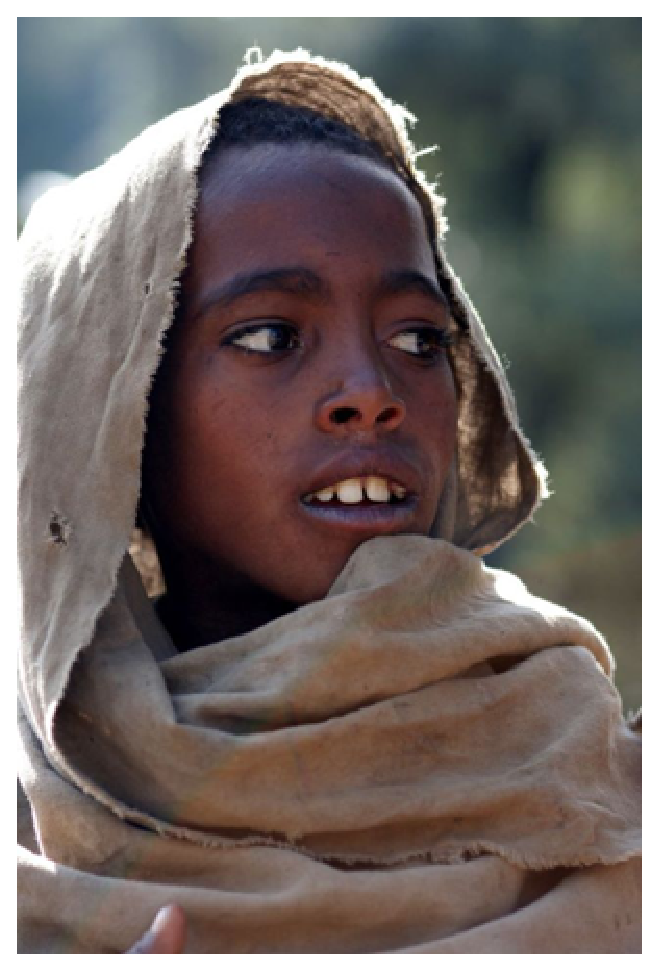
\includegraphics[]{etiopan.eps}}\,\reflectbox{\scalebox{0.45}{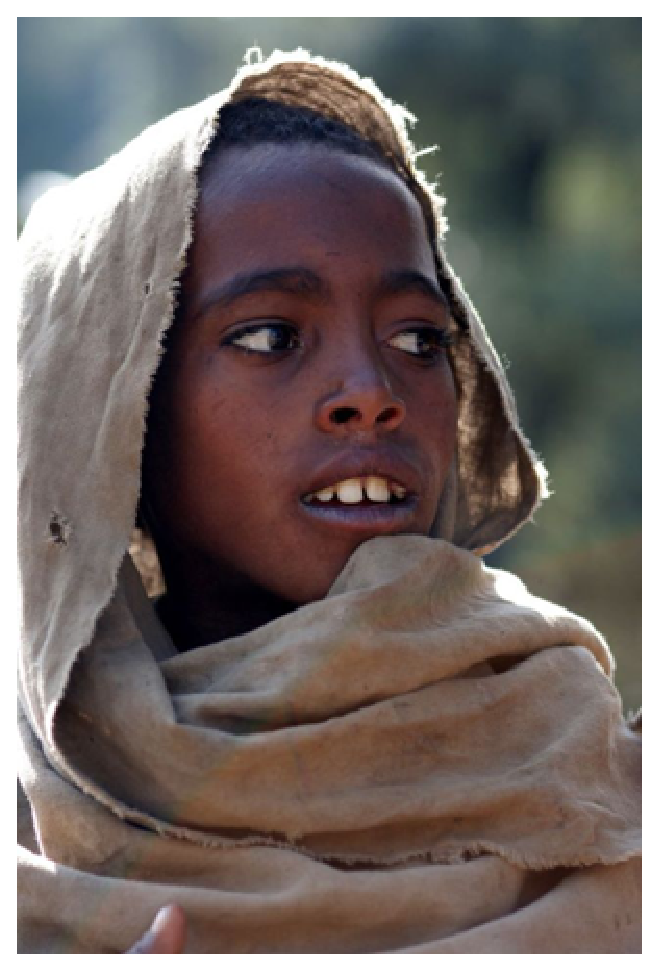
\includegraphics[]{etiopan.eps}}}
    \caption{Malý Etiopánek a jeho bratříček.}
    %%\scalebox{0.45}{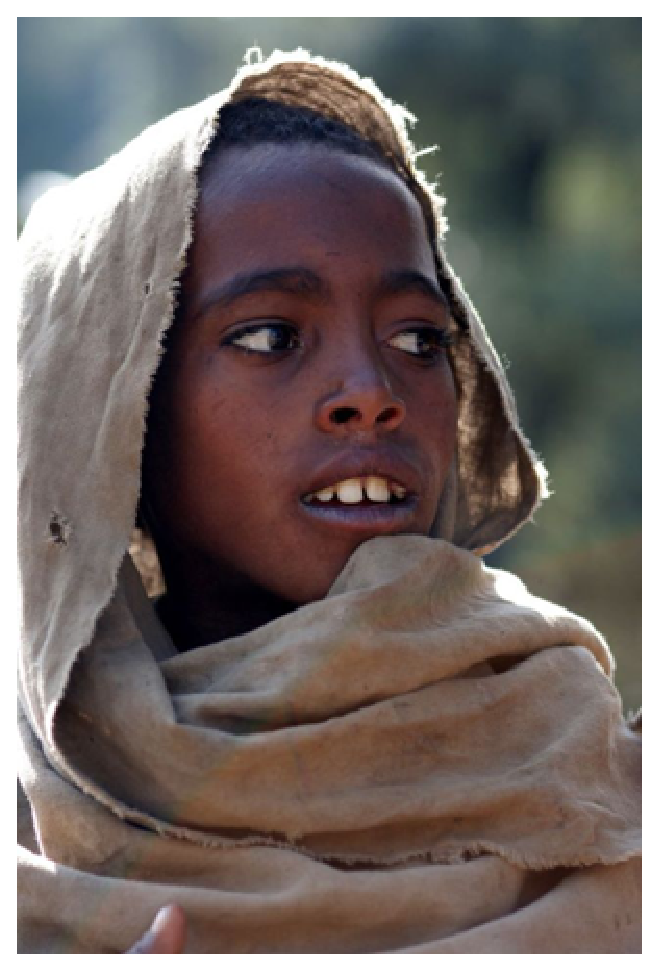
\includegraphics[]{etiopan.eps}}\,\reflectbox{\scalebox{0.45}{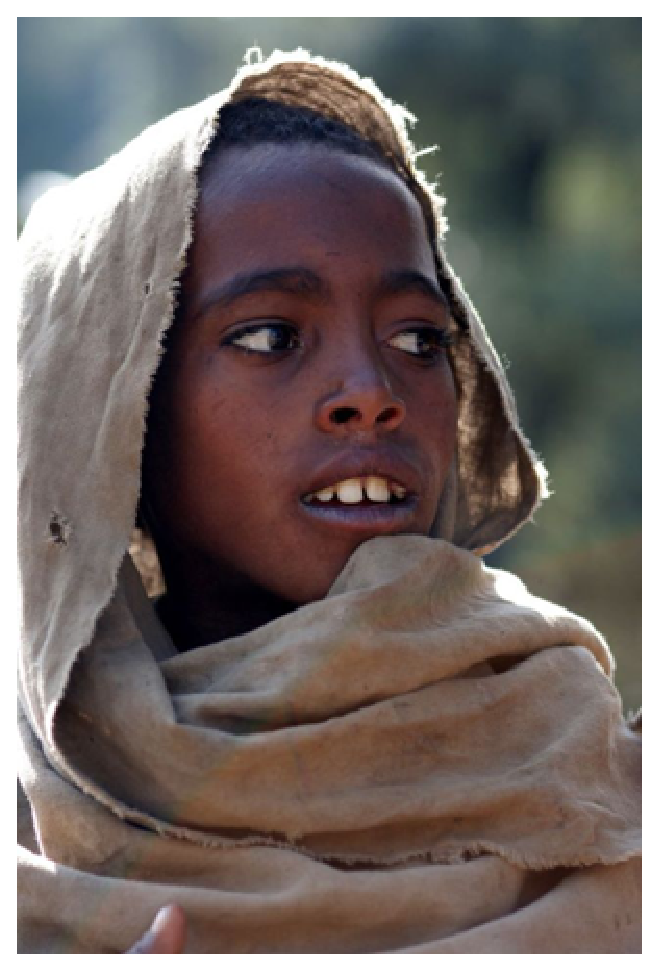
\includegraphics[]{etiopan.eps}}}
    %%\caption{Siamské dvojčatá z Etiópie, jedno z nich sa nedožije ďalšieho roka.}
    \label{img:img1}
    \end{center}
\end{figure}
\newpage
\noindent Rozdíl mezi vektorovým $\dots$

\begin{figure}[ht]
    \centering
    \scalebox{0.4}{
\includegraphics{oniisan.eps}}
    \caption{Vektorový obrázek}
    \label{fig:img2}
\end{figure}

\noindent $\dots$ a bitmapovým obrázkem
\begin{figure}[ht]
    \centering
    \scalebox{0.6}{
\includegraphics{oniisan2.eps}}
    \caption{Bitmapový obrázek}
    \label{fig:img3}
\end{figure}

\noindent se projeví například při zvětšení.

Odkazy (nejen ty) na obrázky \ref{img:img1}, \ref{fig:img2} a \ref{fig:img3}, na tabulky \ref{tab:fiat} a \ref{tab:kleen} a také na algoritmus \ref{alg:FSM} jsou udělány pomocí krížových odkazů. Pak je ovšem potřeba zdrojový soubor preložit dvakrát.

Vektorové obrázky lze vytvořit i přímo v~\LaTeX u, například pomocí prostředí \texttt{picture}.\
\newpage
\begin{landscape}
\begin{figure}
    \centering
    \begin{picture}(600,300)
        \framebox(600,300)[0,0]
        {   
            \linethickness{0.2mm}
            %%% BASE
            \put(-250,-240){\line(1,0){450}} %front
            \put(-250,-240){\line(0,1){10}} %front
            \put(-250,-230){\line(1,0){275}} %front
            \put(-250,-230){\line(2,1){70}} %side

            \put(-80,-240){\line(0,1){7}}
            \put(-84,-240){\line(0,1){7}}
            \put(-88,-240){\line(0,1){7}}
            \put(-92,-240){\line(0,1){7}}
            \put(-96,-240){\line(0,1){7}}
            \put(-100,-240){\line(0,1){7}}
            \put(-100,-236){\oval(40,7)}
            \put(-104,-240){\line(0,1){7}}
            \put(-108,-240){\line(0,1){7}}
            \put(-112,-240){\line(0,1){7}}
            \put(-116,-240){\line(0,1){7}}
            
            \put(200,-240){\line(2,1){100}}
            \put(200,-230){\line(2,1){100}}
            \put(200,-240){\line(0,1){10}}
            
            \put(25,-240){\line(0,1){10}} %fgar
            %\put(25,-240){\line(1,1){20}} %fgar
            \put(25,-240){\qbezier[100](0,0)(17,14)(35,28)}
            \put(125,-230){\line(1,0){75}}
            \put(125,-240){\line(0,1){10}}
            \put(25,-230){\line(2,1){35}}
            \put(125,-230){\line(2,1){35}} %garfrontvert
            
            \put(235,-180){\line(1,0){65}}
            \put(-101,-180){\line(1,0){51}}
            
            %% HOUSE
            \put(-180,-212){\line(1,0){30}}
            \put(0,-212){\line(1,0){60}}
            \put(160,-212){\line(1,0){30}}
            \put(-180,-212){\line(0,1){161}}
            \put(-150,-212){\line(0,1){75}} %pillar
            \put(-150,-212){\line(2,1){10}} %side
            \put(-140,-207){\line(0,1){70}} %pillar
            \put(-102,-188){\line(0,1){51}} %pillar back
            \put(-112,-193){\line(0,1){56}} %pillar back
            \put(-135,-193){\line(0,1){56}} %pillar back
            \put(-135,-193){\line(1,0){23}} %pillar back
            \put(-112,-193){\line(2,1){10}} %side
            \put(-150,-137){\line(1,0){150}}
            \put(0,-212){\line(0,1){75}}
            \put(190,-212){\line(2,1){45}} % horizontal side
            \put(190,-212){\line(0,1){119}} % vertical side
            \put(190,-110){\line(2,1){45}} % horizontal side
            \put(235,-190){\line(0,1){120}} % vertical side back
            %% SEC FLOOR
            %WINDOW
            \put(-160,-60){\line(1,0){160}}
            \put(-160,-115){\line(0,1){55}} 
            \put(-160,-115){\line(1,0){160}}
            \put(0,-115){\line(0,1){55}} 
            
            \put(-80,-100){\line(1,1){10}}
            \put(-83,-100){\line(1,1){10}}
            
            \put(-120,-80){\line(1,1){10}}
            \put(-123,-80){\line(1,1){10}}
            %wOOF
            \put(-180,-51){\line(1,0){190}} 
            \put(95,-51){\line(2,1){45}} %side
            \put(-180,-51){\line(2,1){46}} %side
            \put(-134,-28){\line(1,0){190}} 
            \put(10,-51){\line(2,1){45}} %side
            
            \put(10,-50){\qbezier[500](0,-1)(20, -20)(87, 0)}
            \put(54,-28){\qbezier[500](2,0)(20, -20)(86, 0)}
            
            %BALCONY
            \put(10,-110){\line(2,1){45}} % horizontal side
            \put(55,-87){\line(0,1){28}}
            \put(10,-110){\line(0,1){58}}
            \put(20,-105){\line(0,1){48}} %%doors to balcony
            \put(45,-92){\line(0,1){32}} %%doors to balcony
            \put(28,-80){\line(1,1){10}}
            \put(31,-80){\line(1,1){10}}
            
            \put(10,-93){\line(1,0){82}} %rails top front
            \put(95,-93){\line(1,0){95}} %rails top front
            \put(10,-110){\line(1,0){180}} %rails bot front
            
            \put(55,-70){\line(1,0){79}} %rails top back
            \put(140,-70){\line(1,0){95}} %rails top back
            \put(55,-87){\line(1,0){180}} %rails bot back
            
            \put(70,-85){\line(1,1){10}}
            \put(73,-85){\line(1,1){10}}
            
            \put(110,-105){\line(1,1){10}}
            \put(113,-105){\line(1,1){10}}
            
            \put(210,-95){\line(1,1){10}}
            \put(213,-95){\line(1,1){10}}
            
            \put(92,-110){\line(0,1){58}} %%pillar
            \put(95,-110){\line(0,1){59}} %%pillar
            \put(98,-110){\line(0,1){60}} %%pillar
            \put(140,-87){\line(0,1){59}} %%pillarback
            \put(137,-89){\line(0,1){59}} %%pillarback
            \put(134,-89){\line(0,1){57}} %%pillarback
            \put(190,-93){\line(2,1){45}} % horizontal side
            %% GARAGE
            \put(60,-212){\line(0,1){75}}
            \put(160,-212){\line(0,1){75}}
            \put(60,-137){\line(1,0){100}}
            \put(60,-150){\line(1,0){100}}
            \put(60,-160){\line(1,0){100}}
            \put(60,-170){\line(1,0){100}}
            \put(60,-180){\line(1,0){100}}
            \put(60,-190){\line(1,0){100}}
            \put(60,-200){\line(1,0){100}}
            %% STAIRS
            \put(-50,-200){\line(1,0){50}}
            \put(-50,-200){\line(0,1){20}}
            \put(-50,-180){\line(2,1){50}}
            %% Moon awooo
            \put(-300,-50){\qbezier[200](70,-40)(0,-20)(70,40)}
            \put(-300,-50){\qbezier[200](70, -40)(20, -20)(70, 40)}
            %% stars
            \put(-200,7){\circle*{3}}
            \put(-160,-3){\circle*{1}}
            \put(-150,6){\circle*{2}}
            \put(-140,-9){\circle*{1}}
            \put(-70,-4){\circle*{2}}
            \put(-60,2){\circle*{2}}
            \put(-50,-3){\circle*{2}}
            \put(-20,4){\circle*{3}}
            \put(-10,-5){\circle*{3}}
            \put(10,-8){\circle*{2}}
            \put(20,4){\circle*{2}}
            \put(30,2){\circle*{2}}
            \put(40,-3){\circle*{2}}
            \put(50,6){\circle*{1}}
            \put(110,-7){\circle*{2}}
            \put(130,-4){\circle*{3}}
            \put(140,-7){\circle*{2}}
            \put(160,-4){\circle*{1}}
            \put(160,6){\circle*{2}}
            \put(170,0){\circle*{3}}
            \put(180,4){\circle*{1}}
            \put(250,6){\circle*{3}}
            \put(120,5){\circle*{2}}
            \put(150,5){\circle*{3}}
            \put(290,-6){\circle*{1}}
            \put(270,-20){\circle*{2}}
            \put(260,-30){\circle*{3}}
            \put(250,-40){\circle*{1}}
            \put(240,-45){\circle*{2}}
            \put(230,-50){\circle*{3}}
            \put(220,-30){\circle*{1}}
            \put(210,-20){\circle*{2}}
            \put(200,-10){\circle*{3}}
            \put(190,-40){\circle*{1}}
            \put(180,-45){\circle*{2}}
            \put(170,-50){\circle*{3}}
            \put(160,-30){\circle*{1}}
            \put(150,-20){\circle*{2}}
        }
    \end{picture}
    \caption{Vektorový obrázek moderního bydlení vhodného pro 21. století. (Buď to vytvořte stejný obrázek, anebo nakreslete pomocí picture váš vlastní domov.)}
    \label{fig:img4dom}
\end{figure}
\end{landscape}
\end{document}
